% !Mode:: "TeX:UTF-8"
\part{综合运用}
\label{part:ai_exercise}

\newpage

%二维码
\begin{center}{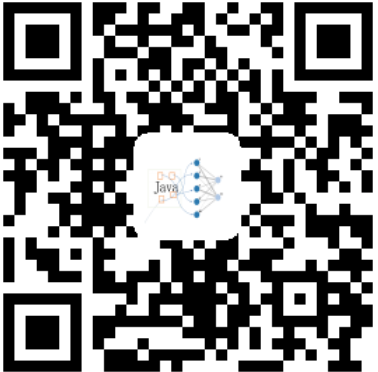
\includegraphics[width=3cm]{barcode.png}}\end{center}\par

十年前,\emph{手写识别}还只是专业技术人员的玩物,而如今\emph{手写识别}已经变成深度学习的入门教程。
而\emph{模式识别}(Pattern Recognition)意味着需要专业人员提供很多特征。
模式识别从19世纪50年代开始出现,在20世纪80年代左右曾经风靡一时,也是信息科学和人工智能的重要组成部分。
它被应用于图像分析与处理、语音识别、数据挖掘等很多方面。
尽管模式识别也很高大上,也有了较长时间的应用,但效果一直差强人意。

这种由人提取特征交给机器,再交给机器去判断的方法识别率一直差强人意。
而\emph{机器学习}可以从海量数据学习\emph{特征},使用已知经验数据(样本)自己提炼特征。
另外,再强调一下概念,深度学习只是机器学习算法的一种,而人工智能也不限于机器学习一种。

\begin{figure}[!htb] \centering
\begin{tikzpicture}
\node(learning) [draw, rectangle] at (2,0) {学习};
\node(knowledge) [draw, ellipse] at(2,1.5) {经验};
\draw[->](0,0) node[left]{新数据} -- node[above]{输入} (learning);
\draw[->](learning) -- node[above]{预测} (4,0) node[right]{人工智能};
\draw[->](knowledge) -- (learning);
\end{tikzpicture}
\end{figure}

大数据和深度学习,让我们能够摆脱人工特征提取的繁琐和束缚,让更多的人参与人工智能并为社会创造价值。
互联网+没有过时,再加上分布式和云计算,使得\emph{人工智能+}如鱼得水,再次迎来十年兴盛,相信接下来是数据为王的时代!

\chapter{大数据和分布式}
\label{chap:java_ex_cloud}

\section{云计算}

云计算是基于互联网的一种全新的模式。通过“云”我们可以轻松地存储数据,运行应用,
甚至进行强度很大的运算。云计算实质上实现了对计算机资源的完全掌控,
我们可以很轻易地通过云对资源进行分配,例如分配内存、处理器等计算资源。

机器学习和云计算、大数据的关系十分密切。大数据技术具有大量的数据与资源,能促进
机器学习的进一步发展。反过来,机器学习的发展也能促进数据挖掘,分析等方面
的进步。

\section{边缘计算}
边缘计算的定义是在靠近数据生成的设备端,就近提供服务。相比于云计算需要
将所有数据上传至云端的特性,边缘计算具有天然的优势。第一,由于边缘计算强调
“边缘”,数据的处理相比于云计算更为实时,高效;第二,边缘计算处理的数据多为
“小数据”,在数据存储和计算上成本都比较低;第三,边缘计算的出现降低了
对网络带宽的需求。随着物联网的不断发展,越来越多的联网设备将出现在
我们的生活中,这大大增加了网络传输的压力。边缘计算则通过数据本地处理
解决了这一问题。

边缘计算是对云计算的一种补充与完善。思科预计到2022年,移动设备和连接数量将达到123亿
\footnote{数据来源思科官网《思科移动网络VNI预测(2017-2022 年)》}。如果仅仅用
云计算来解决这么多互联设备的数据量往往会造成资源浪费,及时性较差,以及隐私泄露
等问题。边缘计算在一方面能减轻云端的负担,另一方面也能保护用户的隐私,具有重要
的实际意义。

\section{开源架构}
随着云计算和大数据的不断发展,人们对于数据存储和数据处理的效率
提出了越来越严格的要求,因此一批优秀的开源架构应运而生。

\subsection{Hadoop}
Hadoop是基于分布式计算的大数据开源架构,它的特点在于能高效,可靠地对
大量数据进行处理。Hadoop由HDFS和MapReduce组成,分别负责数据的分布式
储存和分布式计算。

HDFS提供了大规模存储的分布式解决方案,可以横跨成千上百台机器,操作却像对本地文件
进行操作一样简单,并能存储TB甚至PB级别的特大文件。这些优势来源于在HDFS中,
文件的储存是以较大的抽象块为单位,这样做的好处在于能将文件存储于
不同的硬盘中,使得文件的大小不受限于硬盘大小;同时较大的抽象块有利于对大型
文件进行寻址操作,最小化寻址开销。

除了抽象块,HDFS还包含了NameNode和DataNode。用户在用HDFS进行存储时,客户端首先
会将文件切块,再由DataNode储存在多个硬盘中。同时,NameNode负责记录每一个
文件的切块信息,以及每一块具体的存储机器。这样的系统就构成了NameNode为主服务器,多个
DataNode为从服务器的HDFS文件系统。

MapReduce是Hadoop的计算框架,能够以容错、可靠的方式并行处理海量的数据。
MapReduce主要包括了两个主要部分:Map阶段和Reduce阶段。



\subsection{Storm}
Storm是类似于Hadoop的实时数据处理框架,两者的区别在于Storm用于数据
的实时计算,Hadoop用于对离线数据进行处理。同时,Storm将数据存储在
内存中,这也有区别于Hadoop的HDFS存储方式。Storm也提供了类似于MapReduce
的简单编程模型,便于进行开发。

一个完整的Storm集群应该包括Nimbus,Zookeeper和Supervisor,工作架构
如图\ref{storm_framework}所示。其中,Nimbus负责接受客户端传来的拓扑代码
并分拆task,Zookeeper负责Nimbus和Supervisor之间的通信和协调,Supervisor
接收并处理数据。这样高效的工作架构使得Storm具有实时处理大批量数据的能力,
同时具有高扩展性,可以通过增加节点实现性能的线性提高。

~~~~
\begin{figure}[!ht]
\begin{center}
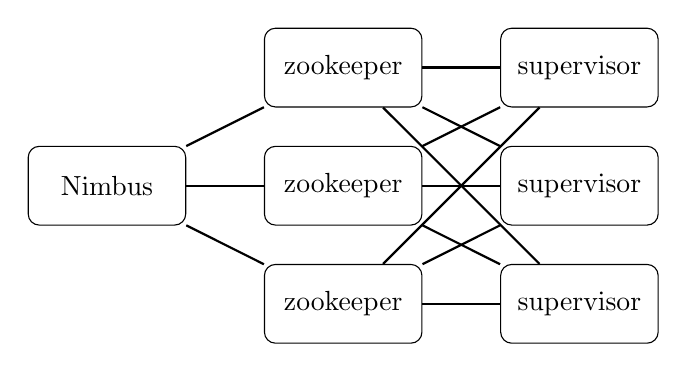
\begin{tikzpicture}
\tikzstyle{arrow} = [thick, -, >= stealth]
\tikzstyle{node} = [rectangle, rounded corners, minimum width = 2cm, minimum height=1cm,text centered, draw = black]
\node[node](Nimbus){Nimbus};
\node[node, right of = Nimbus, xshift = 2cm](zookeeper2){zookeeper};
\node[node, below of = zookeeper2, yshift = -0.5cm](zookeeper3){zookeeper};
\node[node, below of = zookeeper2, yshift = 2.5cm](zookeeper1){zookeeper};
\node[node, right of = zookeeper1, xshift = 2cm](supervisor1){supervisor};
\node[node, right of = zookeeper2, xshift = 2cm](supervisor2){supervisor};
\node[node, right of = zookeeper3, xshift = 2cm](supervisor3){supervisor};
\draw[arrow] (Nimbus)--(zookeeper1);
\draw[arrow] (Nimbus)--(zookeeper2);
\draw[arrow] (Nimbus)--(zookeeper3);
\draw[arrow] (zookeeper1)--(supervisor1);
\draw[arrow] (zookeeper1)--(supervisor2);
\draw[arrow] (zookeeper1)--(supervisor3);
\draw[arrow] (zookeeper2)--(supervisor1);
\draw[arrow] (zookeeper2)--(supervisor2);
\draw[arrow] (zookeeper2)--(supervisor3);
\draw[arrow] (zookeeper3)--(supervisor1);
\draw[arrow] (zookeeper3)--(supervisor2);
\draw[arrow] (zookeeper3)--(supervisor3);
\end{tikzpicture}
\caption{Storm架构示意图}
\label{storm_framework}
\end{center}
\end{figure}

\subsection{Spark}
Spark是一种通用的大数据计算框架,与Hadoop的MapReduce,Storm的
流式实时计算引擎十分相似。同时Spark也提供了大数据和机器学习方面的
框架,逐渐形成了大数据处理的一站式解决平台。

Spark的特点是支持大型,低延迟的数据处理方式。拓展了常用的MapReduce计算
模型。由于Spark支持在内存中进行计算,在必要时依赖硬盘进行复杂运算,因此
Spark比MapReduce更高效。

Spark是MapReduce的一种替代方案,兼容HDFS,Hive等存储方案,能够方便
地融入Hadoop的生态环境,以弥补MapReduce的不足。

\section{示例:人脸识别}



\chapter{车牌识别}
\label{chap:java_ex_recongnition}


手写识别机器学习领域中的一个经典问题。自从深度学习的兴起,MNIST已经是一个被”嚼烂”了的数据集。
该问题要解决的是把28x28像素的灰度手写数字图片,识别为0到9的数字。
而\emph{手写算式识别}在数字识别的基础上,需要识别运算符号,并输出计算结果。

\begin{figure}[!htb]
\centerline{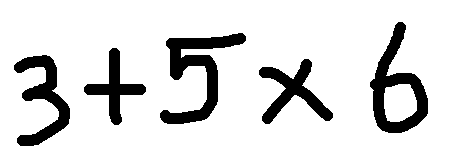
\includegraphics[width=.1\figwidth]{images/handwriting_math.png} $\to$ 识别: $3+5 \times 6$} 
\label{fig:part4_handwriting_math}
\caption{手写算式识别}
\end{figure}

限于篇幅和笔者能力,本演示代码仅支持四则运算($+ - \times \div$),其它运算符号留给同学们研究。
利用深度学习算法,为用户提供手写算式识别,可以极大的提高用户体验。
目前,有很多成熟的产品可以借鉴,相关的论文也非常多。

手写数字识别属于图像分类,可用的算法有:KNN、SVM、BP和CNN。
其中KNN和SVM比较善于数据挖掘,用做手写数字识别的话,比较难达到实用目的;
而BP使用全连接,难于构建深度网络,并存在梯度消失和过拟合问题。
本章例子,选用CNN深度学习训练手写算式识别。

\begin{figure}[!htb] \centering 
\begin{tikzpicture}
\node at (0,0) {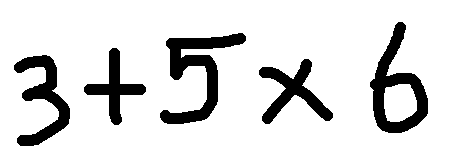
\includegraphics[width=5cm,height=2cm]{images/handwriting_math.png}};
\draw (-2.5,1) rectangle (-1.6,-1);
\draw (-1.6,1) rectangle (-0.8,-1);
\draw (-0.8,1) rectangle (0.3,-1);
\draw (0.3,1) rectangle (1.3,-1);
\draw (1.3,1) rectangle (2.4,-1);
\end{tikzpicture}
\end{figure}

现在我们要识别一个算式,其实和MINIST数字识别没有太多差别,主要是增加了图像切割和四则运算符的识别任务。
为了降低难度,约束字符之间最好有一些间距,不要字符连笔。


\section{图像切割}
手写算式的输入的形式,有2种:拍照、手绘。照片要经过图像处理之后,才能进行切割;
而手绘可直接采集像素轨迹,就省掉了这一步。对于照片的预处理,需要先二值化和降噪把手写数字区域保留下来。
如果考虑图片的背景干扰,可先使用Canny算子检测边缘,这借助OpenCV的API很容易实现。

我们这种要求手写数字不黏连的情况,把Canny输出的图像往X轴投影,就能得出每个数字的横向宽度坐标。
虽然要求数字不黏连,但难保有横向重叠的情况,必须用类似\emph{范水法}进行切割。

\begin{figure}[!htb] \centering 
\begin{tikzpicture}
\node at (0,0) {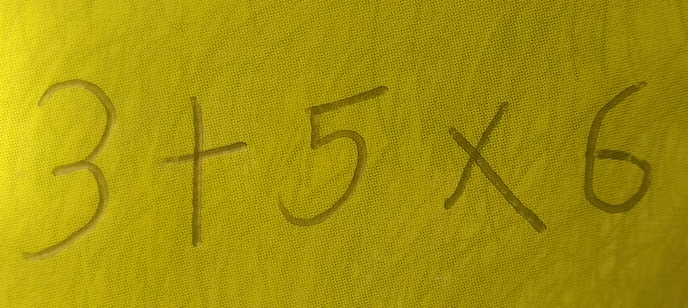
\includegraphics[width=5cm]{images/handwriting_input.png}};
\node at (6,0) {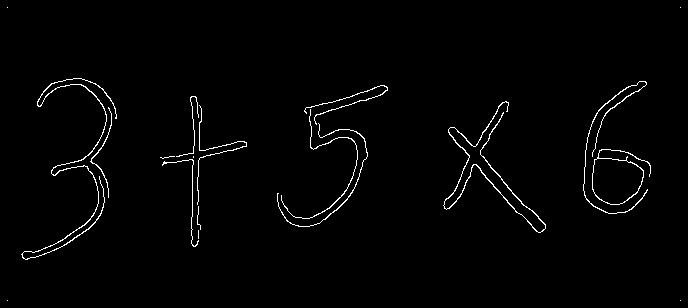
\includegraphics[width=5cm]{images/handwriting_out.png}};
\end{tikzpicture}
\caption{图像处理:二值化和边缘识别(OpenCV)}
\end{figure}

\noindent
这种图像预处理,OpenCV\footnote{OpenCV是一个开源的跨平台视觉库,实现了图像处理和计算机视觉方面的很多通用算法,
支持Linux、Windows、Android和Mac OS操作系统上。
它轻量且高效,同时提供C++、Python、MATLAB等语言的接口。}非常擅长,不需要使用机器学习算法。


\noindent
\emph{Java代码:}
\begin{lstlisting}[language=Java]
System.loadLibrary(Core.NATIVE_LIBRARY_NAME);
Mat img = Imgcodecs.imread(src);
Imgproc.cvtColor(img, img, Imgproc.COLOR_BGR2GRAY);
Imgproc.Canny(img, img, threshold, threshold * 3, 3, true);
Imgcodecs.imwrite(dstImg, img);
\end{lstlisting}

\noindent
\emph{Python代码:}
\begin{lstlisting}[language=Python]
import cv2
from matplotlib import pyplot as plt

img = cv2.imread("handwriting_input.png", 0)
edges = cv2.Canny(img, 30, 60)
plt.subplot(1,2,1), plt.imshow(img, cmap='gray')
plt.title('Original Image'), plt.xticks([]), plt.yticks([])
plt.subplot(1,2,2), plt.imshow(edges, cmap='gray')
plt.title('Edge Image'), plt.xticks([]), plt.yticks([])
plt.show()
\end{lstlisting}

\noindent
实现Canny算子不在本书讨论范围,GitHub上的一份Java实现接近OpenCV的效果
\href{https://github.com/enzoftware/images-processing/blob/master/algorithms/Canny%20Filter/src/com/company/CannyFilter.java}
{\srclink{Github}上获取。}而CSDN上的一份实现简化了很多处理细节,有一定差距。有条件的同学,建议使用OpenCV的接口。
遇到的OpenCV问题,也容易在网络上检索。
\vspace{0.3cm}
\hrule
\begin{multicols}{2}
\begin{itemize}
\item[1.]转换为灰度图像
\item[2.]高斯模糊处理
\item[3.]根据梯度计算图像边缘幅值与角度
\item[4.]非最大信号压制处理(边缘细化)
\item[5.]双阈值边缘连接处理
\item[6.]二值化图像输出结果
\end{itemize}
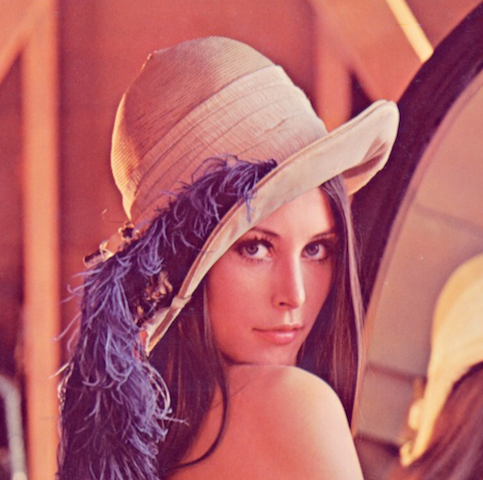
\includegraphics[width=.12\figwidth]{images/Lenna.png}
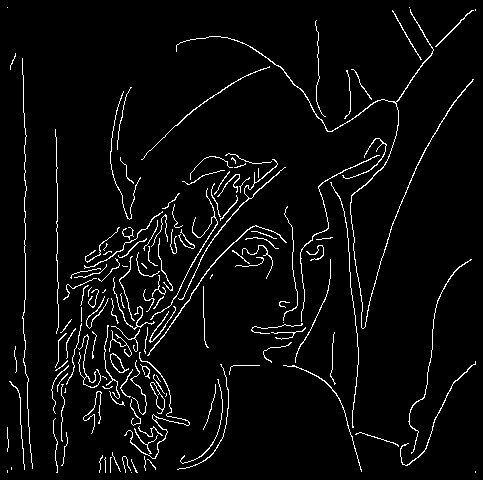
\includegraphics[width=.12\figwidth]{images/Lenna_out.png}
% \end{tabular}
\end{multicols}
\hrule
\ \\
经过Canny算子处理之后,切割图像就非常容易了。把Canny输出的二值图像,在水平方向上投影,对数字进行竖向分割;
同理,在纵向再做一次,就能切割得紧凑一些。以下,是在原图上切割的效果 :

\begin{figure}[!htb] \centering 
\begin{tikzpicture}
\node at (0,0) {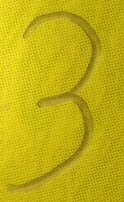
\includegraphics[width=1cm]{images/3.png}};
\node at (2,0) {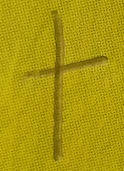
\includegraphics[width=1cm]{images/plus.png}};
\node at (4,0) {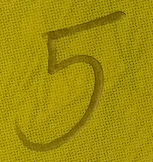
\includegraphics[width=1cm]{images/5.png}};
\node at (6,0) {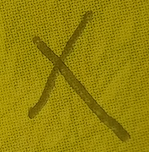
\includegraphics[width=1cm]{images/times.png}};
\node at (8,0) {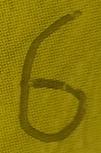
\includegraphics[width=1cm]{images/6.png}};
\end{tikzpicture}
\end{figure}

\noindent
Minist数据集是白底黑字的,使用它训练出来的模型,就很难识别我们的手写算式。所以,有必要在二值图像上切割。
\begin{figure}[!htb] \centering 
\begin{tikzpicture}
\node at (0,0) {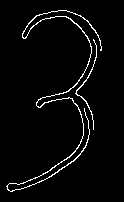
\includegraphics[width=1cm]{images/3_c.png}};
\node at (2,0) {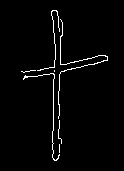
\includegraphics[width=1cm]{images/plus_c.png}};
\node at (4,0) {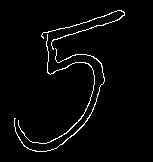
\includegraphics[width=1cm]{images/5_c.png}};
\node at (6,0) {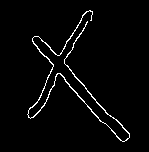
\includegraphics[width=1cm]{images/times_c.png}};
\node at (8,0) {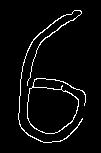
\includegraphics[width=1cm]{images/6_c.png}};
\end{tikzpicture}
\end{figure}

\noindent
但Canny生成的是空心字,并且有很多断线,使用FloodFill算法是填不满的。
笔者采用的是膨胀法,对于每一个\emph{白色点}向周围扩张6个像素,这样的结果还不错,差不多和Minist数据集很接近了。
\begin{figure}[!htb] \centering 
\begin{tikzpicture}
\node at (0,0) {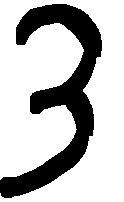
\includegraphics[width=1cm]{images/3_b.png}};
\node at (2,0) {
\includegraphics[width=1cm]{images/plus_b.png}};
\node at (4,0) {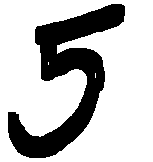
\includegraphics[width=1cm]{images/5_b.png}};
\node at (6,0) {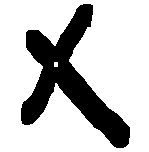
\includegraphics[width=1cm]{images/times_b.png}};
\node at (8,0) {
\includegraphics[width=1cm]{images/6_b.png}};
\end{tikzpicture}
\end{figure}

\noindent
尺寸也要标准化,做成和Minister一样的$28\times28$,这个对图片缩放就可以实现。


\section{算式识别}


\section{结果评估}
\chapter{写诗机器人}
\label{chap:java_ex_poem}

\section{word2vec介绍}
word2vec是google在2013年推出的一个NLP工具,它的特点是将所有的词向量化,这样词与词之间就可以定量的去度量他们之间的关系,挖掘词之间的联系。

\section{如何写诗}


